\documentclass{lessonplan}

% Constants
\newcommand{\lessonNumber}{8}
\title{Lesson \lessonNumber: Trash in the Yard}
\author{\linkHome}
\date{}

% Buildup
\setLessonNumber{\lessonNumber}


%Document
\begin{document}

  \maketitle

  \section{Overview}
    \subsection{Summary}
      This is a fun lesson that allows the kids to use what they've
      learned throughout the year in a fun, semi competitive
      environment, similar to an FLL or FRC event.
    \subsection{Objectives}
    \begin{itemize}
      \item Review simple movement commands
      \item Break down complex tasks and systems into tangible
        objectives
      \item Evaluate performance and iterate
      \item General problem solving skills
      \item (Intermediate) Review claw controls
      \item (Cooperative) Make strategies with other teams
    \end{itemize}
    \subsection{Key Vocabulary Terms}
    \begin{itemize}
      \item Cooperation
    \end{itemize}
    \subsection{Materials}
      \begin{itemize}
        \item Standard ev3 brick
        \item Laptops
        \item Programming Cables
        \item Robot claw attachments (optional)
        \item Large lego pieces, about 20
        \item Lego tires
        \item stopwatch (or equivalent)
      \end{itemize}
  \section{Procedure}
    \subsection{Setup (10 minutes)}
      \paragraph{}
      Setup a robot arena (see appendix B).  A single table should be
      divided into four rectangles along its long axis with tape.
      there should be 4 tires lined up along the middle of the table,
      and 10 miscelaneous large lego pieces distributed evenly around
      each of the two middle quarters.

    \subsection{Introduction (5 minutes)}
      Introduce with a video of a robotics competition (FRC,
      Battlebots, etc.), explain that we are going to be competing in
      a similar fashion

    \subsection{Demonstration (5 minutes)}
      Demonstrate a simple program that pushes a lego piece and
      returns to its original location.  Explain the rules of the
      game: "Trash in the Yard" (appendix B)

    \subsection{Guided Practice (15 mintes)}
      Guide the students through a few practice scenarios in the game,
      make sure to explain that they can use multiple programs and
      switch between them as the game progresses

      \subsubsection{some ideas:}
      \begin{itemize}
        \item teams might need pushing programs of various lengths to
          accomodate differet locations of trash and tires
        \item tires are easiest to get at the beginning of the game.
          can we write a program that gets multiple tires for us?
        \item what about moving out tires to a safer place?
        \item or blocking other robots from getting them?
        \item (Advanced) If the other team is unable to move the
          tires, they might be effective to use as blockades.
      \end{itemize}

    \subsection{Tournament (30 - 40 minutes)}
      Organize the teams, randomly and pit them against each other
      feel free to allow teams to pair up, but make sure teams are
      balanced.  For teams not currently competing, walk them though
      changes that can be made to their programs and strategies.

      \subsubsection{sticking points:}
      \begin{itemize}
        \item Things may get hectic, be prepared for it
        \item You may need to make simple lego structues instead of
          lego parts to make them easier to push around
        \item different teams will have robots with different
          capabilities.  Encourage the students to collaborate with
          each other to use each robot to its fullest potential, and
          avoid letting one robot within a team dominate another.
      \end{itemize}

    \subsection{Conclusion and Evaluation}
      \subsubsection{Exit Questions}
        none, but ask the kids to reflect on what worked in the game and what didn't

    \appendix
    \section{Rules of "Trash in the Yard"} 
    \begin{enumerate}
      \item Rounds will be 90 seconds long, played with teams of 2
        robots each, Each robot within a team is programmed and
        operated by a separate set of students.
      \item Robots must start in the ends of the table, and cannot be
        touched outside this "robot zone" (excepting the rule below),
        doing so, or causing such action to be necessary (driving the
        robot off the end of the table) will incur a penalty of a 10
        second timeout
      \item robots that collide are returned to their respective robot
        zones for free.
      \item Robot operators are not allowed the touch the game pieces
        (the "Trash", and the tires), doing so encures a penalty of 1
        point for trash, and 5 points for tires
      \item operators are not allowed to touch the other team's
        robots, under penalty of 5 points
      \item robot operators cannot touch a robot while it is in
        contact with a tire, doing incurs the 5 point penalty
      \item At the end of the 90 second round, teams will earn 1 point
        for each piece of "trash" in the other team's trash zone, and
        5 points for each tire in their trash zone.  pieces in the
        robot zone are worth no points
      \item pieces that fall off of the table will be placed back on
        it.  Tires will be placed on the opposing side of the
        offending robot, "trash" will be placed on the side of the
        offending robot.
    \end{enumerate}
    \section{The game field}
    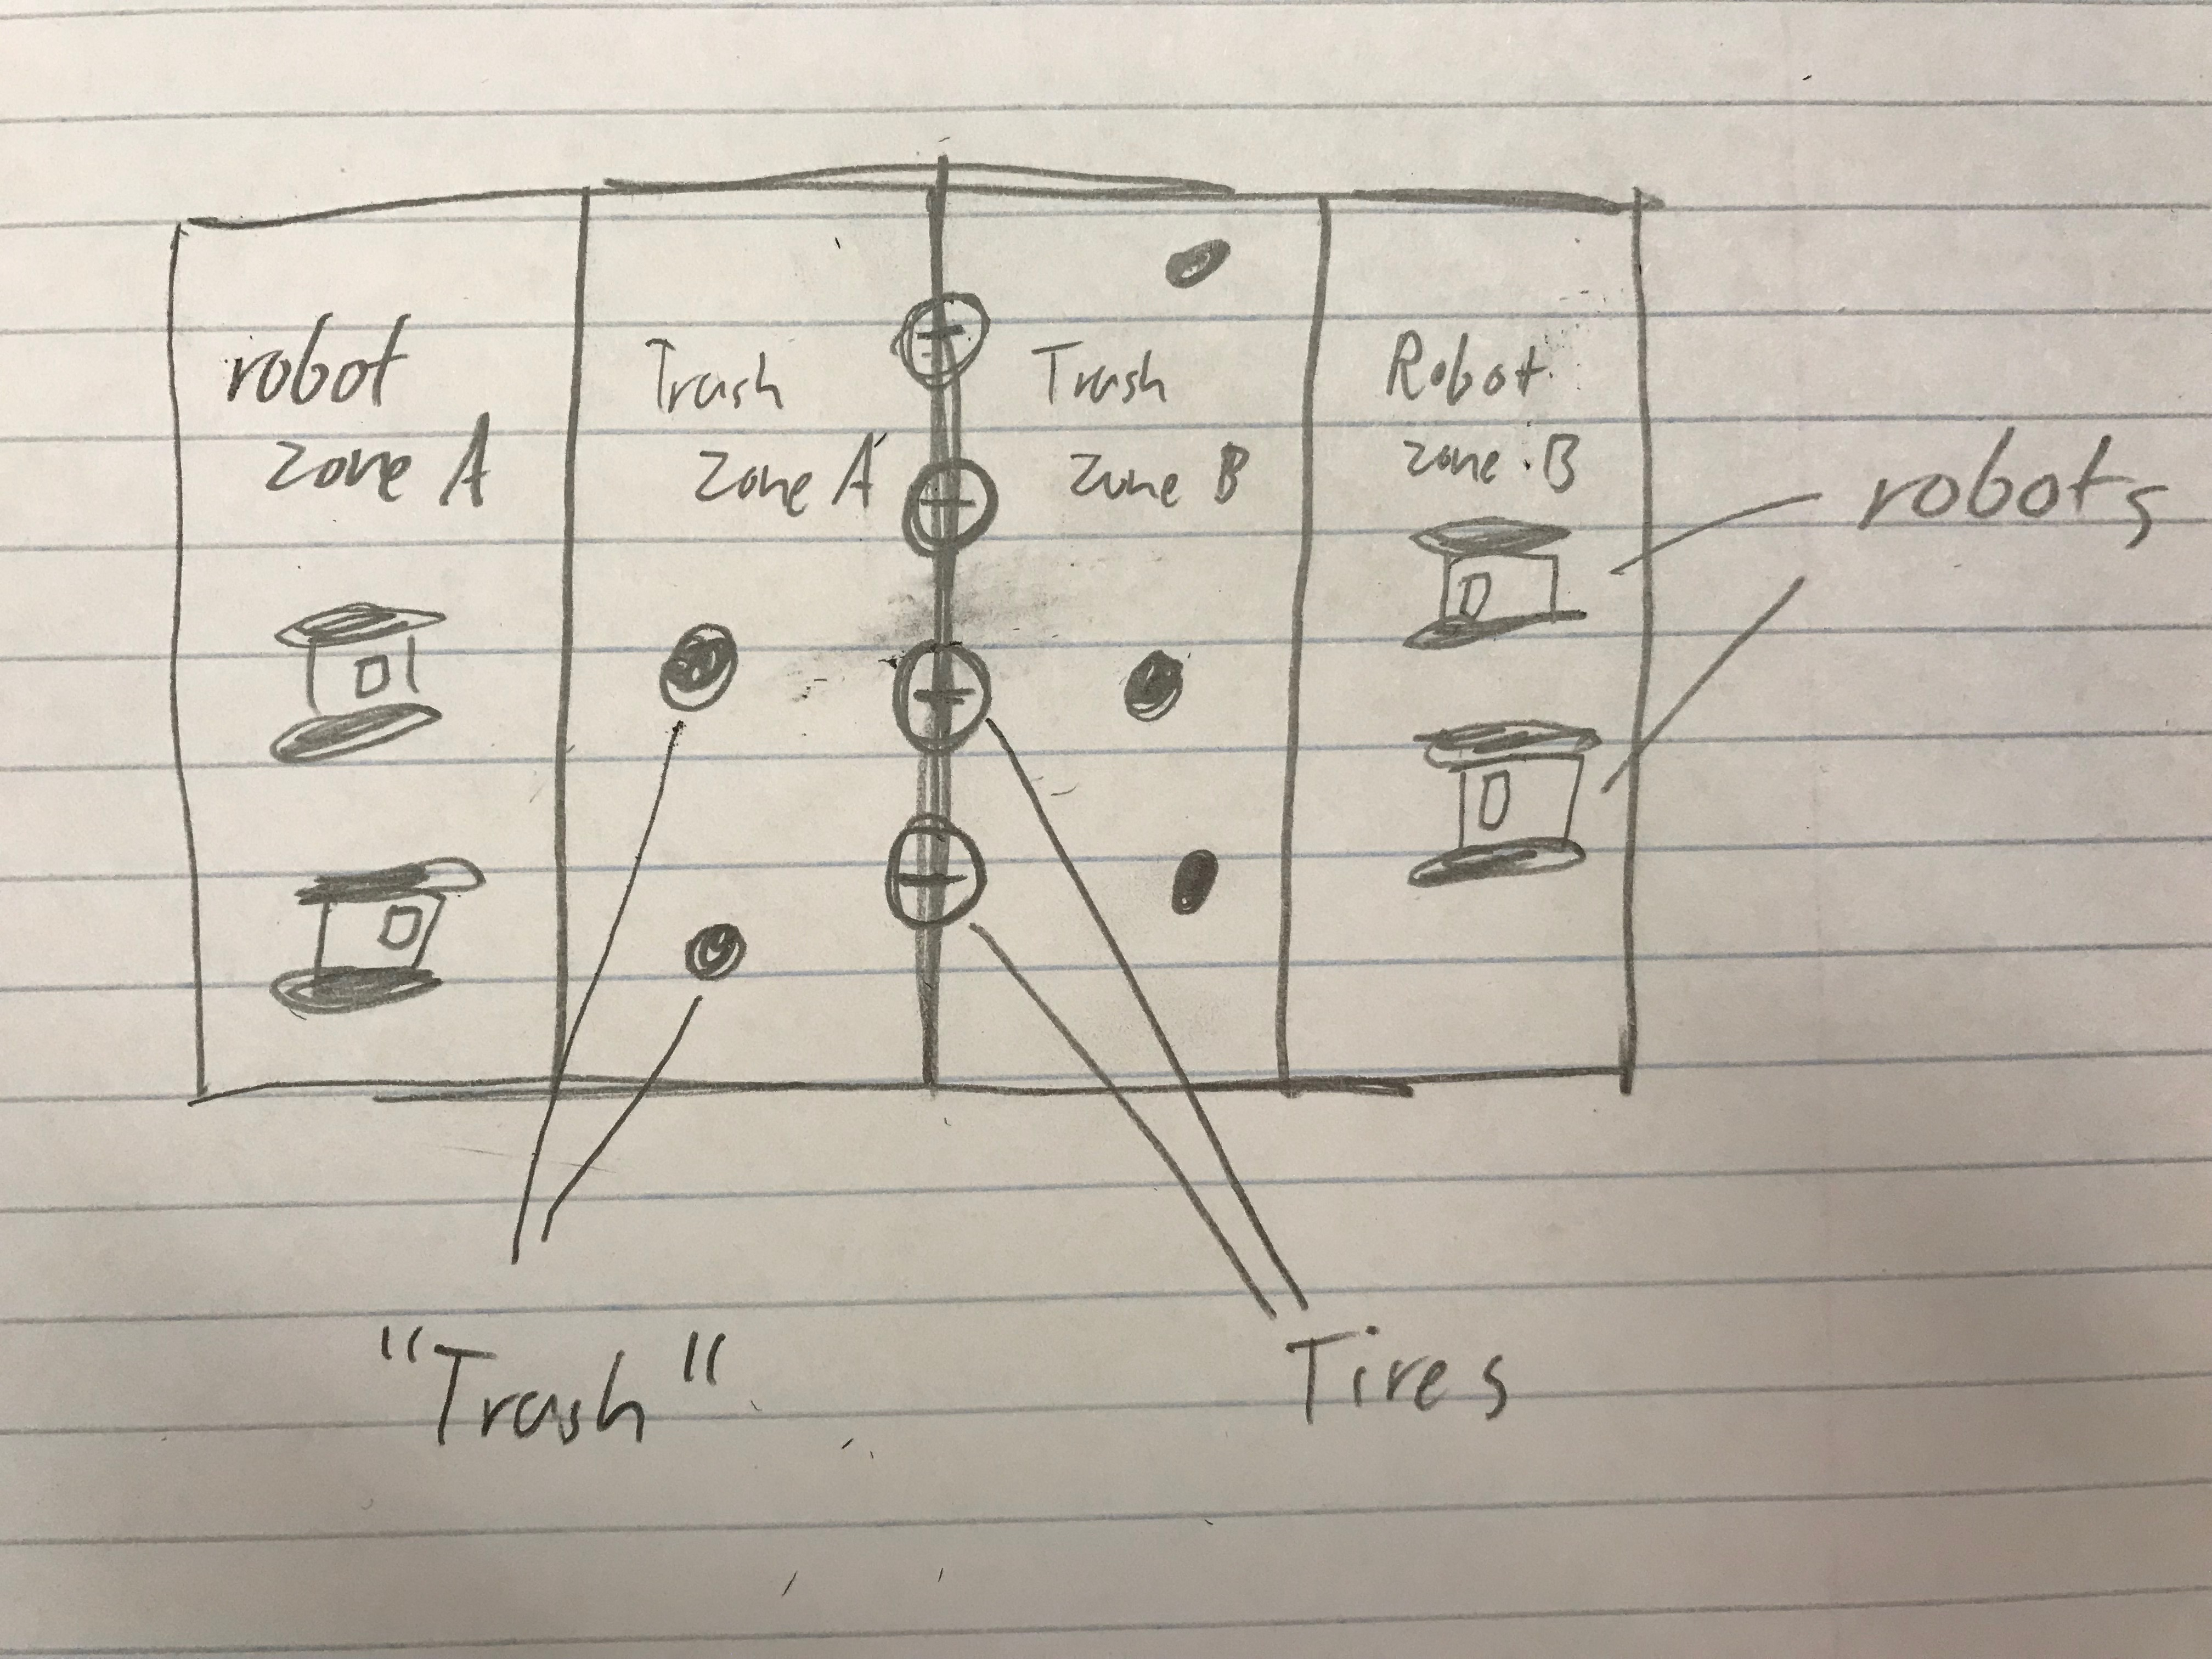
\includegraphics[width=\textwidth]{field.jpeg}
\end{document}
